\documentclass[]{article}
\usepackage{lmodern}
\usepackage{amssymb,amsmath}
\usepackage{ifxetex,ifluatex}
\usepackage{fixltx2e} % provides \textsubscript
\ifnum 0\ifxetex 1\fi\ifluatex 1\fi=0 % if pdftex
  \usepackage[T1]{fontenc}
  \usepackage[utf8]{inputenc}
\else % if luatex or xelatex
  \ifxetex
    \usepackage{mathspec}
  \else
    \usepackage{fontspec}
  \fi
  \defaultfontfeatures{Ligatures=TeX,Scale=MatchLowercase}
\fi
% use upquote if available, for straight quotes in verbatim environments
\IfFileExists{upquote.sty}{\usepackage{upquote}}{}
% use microtype if available
\IfFileExists{microtype.sty}{%
\usepackage{microtype}
\UseMicrotypeSet[protrusion]{basicmath} % disable protrusion for tt fonts
}{}
\usepackage[margin=1in]{geometry}
\usepackage{hyperref}
\hypersetup{unicode=true,
            pdftitle={Tema 3},
            pdfborder={0 0 0},
            breaklinks=true}
\urlstyle{same}  % don't use monospace font for urls
\usepackage{graphicx,grffile}
\makeatletter
\def\maxwidth{\ifdim\Gin@nat@width>\linewidth\linewidth\else\Gin@nat@width\fi}
\def\maxheight{\ifdim\Gin@nat@height>\textheight\textheight\else\Gin@nat@height\fi}
\makeatother
% Scale images if necessary, so that they will not overflow the page
% margins by default, and it is still possible to overwrite the defaults
% using explicit options in \includegraphics[width, height, ...]{}
\setkeys{Gin}{width=\maxwidth,height=\maxheight,keepaspectratio}
\IfFileExists{parskip.sty}{%
\usepackage{parskip}
}{% else
\setlength{\parindent}{0pt}
\setlength{\parskip}{6pt plus 2pt minus 1pt}
}
\setlength{\emergencystretch}{3em}  % prevent overfull lines
\providecommand{\tightlist}{%
  \setlength{\itemsep}{0pt}\setlength{\parskip}{0pt}}
\setcounter{secnumdepth}{0}
% Redefines (sub)paragraphs to behave more like sections
\ifx\paragraph\undefined\else
\let\oldparagraph\paragraph
\renewcommand{\paragraph}[1]{\oldparagraph{#1}\mbox{}}
\fi
\ifx\subparagraph\undefined\else
\let\oldsubparagraph\subparagraph
\renewcommand{\subparagraph}[1]{\oldsubparagraph{#1}\mbox{}}
\fi

%%% Use protect on footnotes to avoid problems with footnotes in titles
\let\rmarkdownfootnote\footnote%
\def\footnote{\protect\rmarkdownfootnote}

%%% Change title format to be more compact
\usepackage{titling}

% Create subtitle command for use in maketitle
\newcommand{\subtitle}[1]{
  \posttitle{
    \begin{center}\large#1\end{center}
    }
}

\setlength{\droptitle}{-2em}
  \title{Tema 3}
  \pretitle{\vspace{\droptitle}\centering\huge}
  \posttitle{\par}
\subtitle{Solutii}
  \author{}
  \preauthor{}\postauthor{}
  \date{}
  \predate{}\postdate{}

%%%%%%%%%%%%%%%%%%%%%%%%%%%%%%%%%%%%%%%%%%%%%%%%%%%%%%%%%%%%%%%%%%%%%%%%%%%%%%%%%%%%%%%%%%%%%%%%%%%%%%%%%%%%%%%%%%%%%
\usepackage{subfigure}
\usepackage{booktabs}
\usepackage{slashbox}

%%%%%%%%%%%%%%%%%%%%%%%%%%%%%%%%%%%%%%%%%%%%%%%%%%%%%%%%%%%%%%%%%%%%%%%%%%%%%%%%%%%%%%%%%%%%%%%%%%%%%%%%%%%%%%%%%%%%%
%CITEVA DEFINITII
\def\om{\omega}
\def\Om{\Omega}
\def\et{\eta}
\def\td{\tilde{\delta}}
\def\m{{\mu}}
\def\n{{\nu}}
\def\k{{\kappa}}
\def\l{{\lambda}}
\def\L{{\Lambda}}
\def\g{{\gamma}}
\def\a{{\alpha}}
\def\e{{\varepsilon}}
\def\b{{\beta}}
\def\G{{\Gamma}}
\def\d{{\delta}}
\def\D{{\Delta}}
\def\t{{\theta}}
\def\s{{\sigma}}
\def\S{{\Sigma}}
\def\z{{\zeta}}
\def\qed{\hfill\Box}
\def\ds{\displaystyle}
\def\mc{\mathcal}
%%%%%%%%%%%%%%%%%%%%%%%%%%%%%%%%%%%%%%%%%%%%%%%%%%%%%%%%%%%%%%%%%%%%%%%%%%%%%%%%%%%%%%%%%%%%%%%%%%%%%%%%%%%%%%%%%%%%%%
\def\1{{\mathbf 1}}
\def\CC{{\mathbb C}}
\def\RR{{\mathbb R}}
\def\QQ{{\mathbb Q}}
\def\ZZ{{\mathbb Z}}
\def\PP{{\mathbb P}}
\def\EE{{\mathbb E}}
\def\VV{{\mathbb V}}
\def\NN{{\mathbb N}}
\def\FF{{\mathbb F}}
%\def\SS{{\mathbb S}}
\def\MO{{\mathcal O}}
\def\MA{{\mathcal A}}
\def\MF{{\mathcal F}}
\def\MR{{\mathcal R}}
\def\MB{{\mathcal B}}
\def\MM{{\mathcal M}}
\def\MN{{\mathcal N}}
\def\MU{{\mathcal U}}
\def\MP{{\mathcal P}}
\def\MS{{\mathcal S}}
\def\MBS{{\mathbf S}}
\def\MX{{\bm{ \mathscr X}}}
%%%%%%%%%%%%%%%%%%%%%%%%%%%%%%%%%%%%%%%%%%%%%%%%%%%%%%%%%%%%%%%%%%%%%%%%%%%%%%%%%%%%%%%%%%%%%%%%%%%%%%%%%%%%%%%%%%%%%
%Header and Footer
\usepackage{fancyhdr}

\pagestyle{fancy}
\fancyhf{}
\rhead{Universitatea din Bucure\c sti\\ Facultatea de Matematic\u a \c si Informatic\u a}
\lhead{\textit{Curs}: Statistic\u a\\ \textit{Instructor}: A. Am\u arioarei}
\rfoot{Pagina \thepage}
\lfoot{Grupele: 301, 311, 321}
%%%%%%%%%%%%%%%%%%%%%%%%%%%%%%%%%%%%%%%

\begin{document}
\maketitle

%%%%%%%%%%%%%%%%%%%%%%%%
\thispagestyle{fancy}

\subsubsection{\texorpdfstring{Exerci\c tiul
1}{Exerciiul 1}}\label{exerciiul-1}

\begin{enumerate}
\def\labelenumi{\alph{enumi})}
\tightlist
\item
  In acest caz probabilitatea pe care o c\u aut\u am este \(\PP(2b)\),
  unde \(2b\) inseamn\u a c\u a a doua bil\u a a fost albastr\u a. Din
  formula probabilit\u a\c tii totale avem:

  \begin{align*}
  \PP(2b)&=\PP(2b|1r)\PP(r)+\PP(2b|1b)\PP(b)\\
  &=\frac{b}{r+b+d}\cdot\frac{r}{r+b}+\frac{b+d}{r+b+d}\cdot\frac{b}{r+b}\\
  &=\frac{b}{b+r}.
  \end{align*}
\item
  Trebuie s\u a calcul\u am probabilitatea:

  \begin{align*}
  \PP(1b|2b)&=\frac{\PP(2b|1b)\PP(1b)}{\PP(2b)}\\
  &=\frac{\frac{b+d}{r+b+d}\cdot\frac{b}{r+b}}{\frac{b}{b+r}}=\frac{b+d}{r+b+d}.
  \end{align*}
\item
  Folosim induc\c tie. Pentru \(n=2\) am v\u azut c\u a propozi\c tia
  este adev\u arat\u a din punctele precedente. S\u a presupunem acum
  c\u a \(\PP(B_k)=\PP(B_1)\) pentru orice \(k\in\{1,2,\dots,n-1\}\)
  \c si vrem s\u a ar\u at\u am c\u a rela\c tia r\u amane
  adev\u arat\u a \c si pentru \(k=n\). Observ\u am c\u a dac\u a
  \(N_k(b)\) reprezint\u a num\u arul de bile albastre la pasul \(k\)
  atunci:

  \begin{align*}
  \PP(B_n)&=\PP(B_n|B_{n-1})\PP(B_{n-1})+\PP(B_n|B_{n-1}^c)\PP(B_{n-1}^c)\\
  &=\frac{N_{n-2}(b)+d}{r+b+(n-1)d}\cdot\frac{b}{r+b}+\frac{N_{n-2}(b)}{r+b+(n-1)d}\cdot\frac{r}{r+b},
  \end{align*}

  unde am folosit pasul de induc\c tie (\(\PP(B_{n-1})=\frac{b}{r+b}\)).
  Folosind din nou ipoteza de induc\c tie avem \[
  \PP(B_{n-2})=\frac{N_{n-2}(b)}{r+b+(n-2)d}=\frac{b}{r+b}
  \] de unde g\u asim \(N_{n-2}(b)=\frac{b}{r+b}\cdot[r+b+(n-2)d]\).
  Inlucuind aceast\u a rela\c tie in expresia lui \(\PP(B_n)\)
  ob\c tinem:

  \begin{align*}
  \PP(B_n)&=\frac{N_{n-2}(b)(b+r)+bd}{(b+r)[r+b+(n-1)d]}\\
  &=\frac{\frac{b}{r+b}\cdot[r+b+(n-2)d](b+r)+bd}{(b+r)[r+b+(n-1)d]}\\
  &=\frac{b[r+b+(n-1)d]}{(b+r)[r+b+(n-1)d]}=\frac{b}{b+r}=\PP(B_1).
  \end{align*}
\item
  Trebuie s\u a g\u asim probabilitatea
  \(\PP(B_1|B_2,\dots B_{n+1})=\frac{\PP(B_1,\dots,B_{n+1})}{\PP(B_2,\dots,B_{n+1})}\).
  Avem din formula probabilit\u a\c tii totale c\u a:

  \begin{align*}
  \PP(B_1,\dots,B_{n+1})&=\PP(B_{n+1}|B_1,\dots,B_n)\PP(B_n|B_1,\dots,B_{n-1})\dots\PP(B_2|B_1)\PP(B_1)\\
  &=\frac{b+nd}{b+r+nd}\cdot\frac{b+(n-1)d}{b+r+(n-1)d}\dots\frac{b+d}{b+r+d}\cdot\frac{b}{b+r}\\
  &=\frac{b(b+d)\dots(b+nd)}{(b+r)(b+r+d)\dots(b+r+nd)}
  \end{align*}

  \c si

  \begin{align*}
  \PP(B_2,\dots,B_{n+1})&=\PP(B_1,B_2,\dots,B_{n+1})+\PP(B_1^c,B_2,\dots,B_{n+1})\\
  &=\PP(B_{n+1}|B_1,\dots,B_n)\PP(B_n|B_1,\dots,B_{n-1})\dots\PP(B_2|B_1)\PP(B_1)+\\
  &+\PP(B_{n+1}|B_1^c,\dots,B_n)\PP(B_n|B_1^c,\dots,B_{n-1})\dots\PP(B_2|B_1^c)\PP(B_1^c)\\
  &=\frac{b+nd}{b+r+nd}\cdot\frac{b+(n-1)d}{b+r+(n-1)d}\dots\frac{b+d}{b+r+d}\cdot\frac{b}{b+r}+\\
  &+\frac{b+(n-1)d}{b+r+nd}\dots\frac{b}{b+r+d}\cdot\frac{r}{b+r}\\
  &=\frac{b(b+d)\dots[b+(n-1)d](b+r+nd)}{(b+r)(b+r+d)\dots(b+r+nd)}.
  \end{align*}

  Observ\u am c\u a

  \begin{align*}
  \PP(B_1|B_2,\dots,B_{n+1})&=\frac{\PP(B_1,\dots,B_{n+1})}{\PP(B_2,\dots,B_{n+1})}\\
  &=\frac{\frac{b(b+d)\dots(b+nd)}{(b+r)(b+r+d)\dots(b+r+nd)}}{\frac{b(b+d)\dots[b+(n-1)d](b+r+nd)}{(b+r)(b+r+d)\dots(b+r+nd)}}\\
  &=\frac{b+nd}{b+r+nd}\to 1.
  \end{align*}
\end{enumerate}

\subsubsection{\texorpdfstring{Exerci\c tiul
2}{Exerciiul 2}}\label{exerciiul-2}

Fie \(N_1\) num\u arul de teste necesare pentru indentificarea primului
tranzistor defect, \c si \(N_2\) num\u arul de teste suplimentare
necesare pentru identificarea celui de-al doilea tranzistor defect. Cum
sunt \(5\) tranzistori avem \(0\leq N_1+N_2\leq 5\). Dac\u a not\u am cu
\(T_s\) al \(s\)-lea tranzistorul, \(1\leq s\leq 5\), avem
\(\PP((T_i,T_j)) = \frac{1}{\binom{2}{5}} = \frac{1}{10}\) deoarece
tranzistorii au aceea\c si \c sans\u a s\u a fie defec\c ti. Prin urmare

\begin{align*}
    \PP(N_1=1,N_2=1) &= \PP((T_1,T_2)) = \frac{1}{10},\\
    \PP(N_1=1,N_2=2) &= \PP((T_1,T_3)) = \frac{1}{10},\\
    \PP(N_1=1,N_2=3) &= \PP((T_1,T_4)\cup(T_1,T_5)) = \frac{2}{10},\, (\mbox{$N_1=1$ \c si $2$, $3$, $4^e$ OK deci $5$ e defect})\\
    \PP(N_1=2,N_2=1) &= \PP((T_2,T_3)) = \frac{1}{10},\\
    \PP(N_1=2,N_2=2) &= \PP((T_2,T_4)\cup(T_2,T_5)) = \frac{2}{10},\, (\mbox{$N_1=2$ \c si $N_2=2$ sau $4$ sau $5$ defecte})\\
    \PP(N_1=3,N_2=1) &= \PP((T_3,T_4)\cup(T_3,T_5)) = \frac{2}{10},\, (\mbox{$N_1=3$ \c si $N_2=1$ sau $4$ sau $5$ defecte})\\
    \PP(N_1=3,N_2=0) &= \PP((T_4,T_5)) = \frac{1}{10},\, (\mbox{$N_1=3$ \c si primele $3$ OK atunci $4$ \c si $5^e$ defecte})
\end{align*}

\begin{center}
\begin{tabular}{c|ccccc}
\toprule
\backslashbox{$N_1$}{$N_2$}& 0 & 1 & 2 & 3 &  $\sum$\\
\midrule
1 & 0 & $\frac{1}{10}$ & $\frac{1}{10}$ & $\frac{2}{10}$ & $\frac{4}{10}$ \\
2 & 0 & $\frac{1}{10}$ & $\frac{2}{10}$ & 0 &  $\frac{3}{10}$\\
3 & $\frac{1}{10}$ & $\frac{2}{10}$ & 0 & 0 &  $\frac{3}{10}$\\
\midrule
$\sum$ & $\frac{1}{10}$  & $\frac{4}{10}$ & $\frac{3}{10}$ & $\frac{2}{10}$ &  \\
\bottomrule
\end{tabular}
\end{center}\par

\noindent
Legea lui \(N_1\) este dat\u a de suma pe linii \c si legea lui \(N_2\)
de suma pe coloane. Astfel

\begin{equation*}
N_1\sim\left(\begin{array}{ccc}
            1 & 2 & 3 \\
            \frac{4}{10} & \frac{3}{10} & \frac{3}{10}
        \end{array}
        \right), \quad\quad
N_2\sim\left(\begin{array}{ccccc}
            0 & 1 & 2 & 3 & 4\\
            \frac{1}{10} & \frac{4}{10} & \frac{3}{10} & \frac{2}{10} & 0
        \end{array}\right).
\end{equation*}

Deci
\(\EE[N_1] = 1\times\frac{4}{10} + 2\times\frac{3}{10} + 3\times\frac{3}{10} = \frac{19}{10}\)
\c si
\(\EE[N_2] = 0\times\frac{1}{10} + 1\times\frac{4}{10} + 2\times\frac{3}{10} + 3\times\frac{2}{10} + 4\times0= \frac{16}{10}\).

\subsubsection{\texorpdfstring{Exerci\c tiul
3}{Exerciiul 3}}\label{exerciiul-3}

\begin{enumerate}
\item Cum $f$ este densitate ea verific\u a rela\c tia $\iint_{\RR^2}f(x_1,x_2)\,dx_1dx_2 = 1$ deci $\iint_{\RR^2}c\1_{D(R)}(x_1,x_2)\,dx_1dx_2 = 1$ de unde $c\times(\pi R^2) = 1$ \c si $c = \frac{1}{\pi R^2}$.

\item Legile marginale ale lui $X_1$ \c si $X_2$ sunt determinate de urm\u atoarele formule: $f_{X_1}(x_1) = \int_{\RR}f(x_1,x_2)\,dx_2$ \c si $f_{X_2}(x_2) = \int_{\RR}f(x_1,x_2)\,dx_1$. Avem
    \begin{align*}
        f_{X_1}(x_1) &= \int_{\RR}f(x_1,x_2)\,dx_2 = \int_{\RR}\frac{1}{\pi R^2}\1_{D(R)}(x_1,x_2)\,dx_2\\
        &= \frac{1}{\pi R^2}\int_{\RR}\1_{[-\sqrt{R^2-x_1^2},\sqrt{R^2-x_1^2}]}(x_2)\1_{[-R,R]}(x_1)\,dx_2\\
        &= \frac{1}{\pi R^2}\1_{[-R,R]}(x_1)\int_{-\sqrt{R^2-x_1^2}}^{\sqrt{R^2-x_1^2}}\,dx_2 = \frac{2\sqrt{R^2-x_1^2}}{\pi R^2}\1_{[-R,R]}(x_1)
    \end{align*}
\c si in mod similar g\u asim 
    \begin{align*}
        f_{X_2}(x_2) &= \int_{\RR}f(x_1,x_2)\,dx_1 = \int_{\RR}\frac{1}{\pi R^2}\1_{D(R)}(x_1,x_2)\,dx_1\\
        &= \frac{1}{\pi R^2}\int_{\RR}\1_{[-\sqrt{R^2-x_2^2},\sqrt{R^2-x_2^2}]}(x_1)\1_{[-R,R]}(x_2)\,dx_1\\
        &= \frac{1}{\pi R^2}\1_{[-R,R]}(x_2)\int_{-\sqrt{R^2-x_2^2}}^{\sqrt{R^2-x_2^2}}\,dx_1 = \frac{2\sqrt{R^2-x_2^2}}{\pi R^2}\1_{[-R,R]}(x_2).
    \end{align*}
\item Observ\u am c\u a distan\c ta de la punctul $(X_1,X_2)$ la $(0,0)$ este $L = \sqrt{X_1^2+X_2^2}$. Pentru a g\u asi probabilitatea $\PP(L\leq a)$putem folosi atat o metod\u a geometric\u a cat \c si una probabilist\u a.
    \par\noindent
    Considera\c tii geometrice: cum $(X_1,X_2)$ este uniform distribuit\u a pe discul $D(R)$ atunci
    \begin{equation*}
        \PP(L\leq a) = \PP((X_1,X_2)\in D(a)) = \frac{\MA(D(a))}{\MA(D(R))} = \frac{\pi a^2}{\pi R^2} = \frac{a^2}{R^2}.
    \end{equation*}
    Considera\c tii probabiliste:
    \begin{align*}
        \PP(L\leq a) &= \EE\left[\1_{\{L\leq a\}}\right] = \EE\left[\1_{\{X_1^2+X_2^2\leq a^2\}}\right] = \iint_{\RR^2}\1_{\{x_1^2+x_2^2\leq a^2\}}(x_1,x_2)f(x_1,x_2)\,dx_1dx_2\\
                &= \frac{1}{\pi R^2}\iint_{\RR^2}\1_{\{x_1^2+x_2^2\leq a^2\}}(x_1,x_2)\1_{D(R)}(x_1,x_2)\,dx_1dx_2 \\
                &= \frac{1}{\pi R^2}\iint_{\RR^2}\1_{\{x_1^2+x_2^2\leq a^2\}}(x_1,x_2)\1_{\{x_1^2+x_2^2\leq R^2\}}(x_1,x_2)\,dx_1dx_2 \\
                &= \frac{1}{\pi R^2}\iint_{\RR^2}\1_{\{x_1^2+x_2^2\leq a^2\}\cap \{x_1^2+x_2^2\leq R^2\}}(x_1,x_2)\,dx_1dx_2\\
                &= \frac{1}{\pi R^2}\iint_{\RR^2}\1_{\{x_1^2+x_2^2\leq a^2\}}(x_1,x_2)\,dx_1dx_2 = \frac{\pi a^2}{\pi R^2}\\
                &= \frac{a^2}{R^2}.
    \end{align*}

Am v\u azut c\u a $F_L(a) = \PP(L\leq a) = \frac{a^2}{R^2},\, \forall a\in[0,R]$ de unde g\u asim c\u a densitatea este $f_L(a) = \frac{d}{da}F_L(a) = \frac{2a}{R^2}\1_{[0,R]}(a)$. Media se calculeaz\u a acum u\c sor
    \begin{equation*}
        \EE[L] = \int_{\RR}af_L(a)\,da = 2\int_{\RR}\frac{a^2}{R^2}\1_{[0,R]}(a)\,da = \frac{2}{R^2}\left[\frac{a^3}{3}\right]_{0}^{R} = \frac{2R}{3}.
    \end{equation*}
\end{enumerate}

\begin{figure}[ht]
\centering
\subfigure[]{%
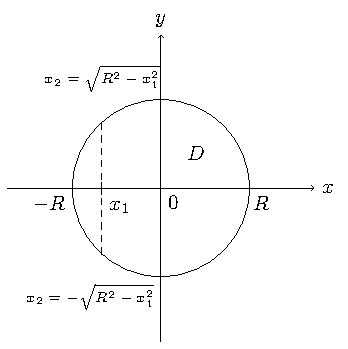
\includegraphics[width=0.25\textwidth]{Figs/Fig1_ex3_t3.pdf}
\label{Fig1_ex3_t3}}
\quad
\subfigure[]{%
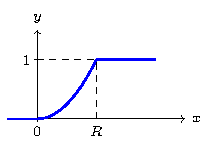
\includegraphics[width=0.5\textwidth]{Figs/Fig2_ex3_t3.pdf}
\label{Fig2_ex3_t3}}
%
\caption{Reprezentarea grafic\u a a lui $D$ \c si func\c tia de reparti\c tie $F_L$}
\label{Fig_ex3_t3}
\end{figure}


\end{document}
